\documentclass[12pt,letter]{article}
\usepackage{geometry}\geometry{top=0.75in}
\usepackage{amsmath}
\usepackage{amssymb}
\usepackage{mathtools}
\usepackage{xcolor} % Color words
\usepackage{cancel} % Crossing parts of equations out
\usepackage{tikz}       % Drawing 
\usetikzlibrary{shapes.geometric, arrows}
\usepackage{pgfplots}   % Other plotting
\usepgfplotslibrary{colormaps,fillbetween}
\usepackage{placeins}   % Float barrier
\usepackage{listings}
\usepackage{enumitem}

% Don't indent
\setlength{\parindent}{0pt}
% Function to replace \section with a problem name specifically formatted
\newcommand{\problem}[1]{\vspace{3mm}\Large\textbf{{Problem
{#1}\vspace{3mm}}}\normalsize\\}
% Formatting function, like \problem
\newcommand{\ppart}[1]{\vspace{2mm}\large\textbf{\\Part
{#1})\vspace{2mm}}\normalsize\\}
% Formatting 
\newcommand{\condition}[1]{\vspace{1mm}\textbf{{#1}:}\normalsize\\}

\begin{document}
\title{CIS 551: Assignment 5}
\author{Steven Walton}
\maketitle
\problem{1: 19.2}
Consider a relation $R$ with five attributes $ABCDE$. You are given the
following dependencies. 
\begin{figure}[ht!]
    \center
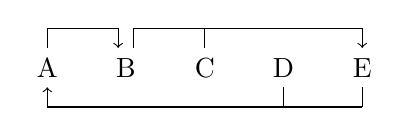
\begin{tikzpicture}
    \node (A) at (0,0) {A};
    \node (B) at (1,0) {B};
    \node (C) at (2,0) {C};
    \node (D) at (3,0) {D};
    \node (E) at (4,0) {E};

    \draw[-] (A) -- (0,0.5);
    \draw[-] (0,0.5) -- (0.9,0.5);
    \draw[->] (0.9,0.5) -- (0.9,0.25);

    \draw[-] (1.1,0.25) -- (1.1,0.5);
    \draw[-] (C) -- (2,0.5);
    \draw[-] (1.1, 0.5) -- (4, 0.5);
    \draw[->] (4, 0.5) -- (4,0.25);

    \draw[-] (E) -- (4, -0.5);
    \draw[-] (D) -- (3, -0.5);
    \draw[-] (4,-0.5) -- (0, -0.5);
    \draw[->] (0,-0.5) -- (0, -0.25);
\end{tikzpicture}
\end{figure}
\ppart{1}
List all keys for R

We can see that $A\rightarrow B$ which means we can rewrite the relationships as
$ACDE$. Giving us

\begin{figure}[ht!]
    \center
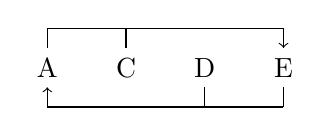
\begin{tikzpicture}
    \node (A) at (0,0) {A};
    \node (C) at (1,0) {C};
    \node (D) at (2,0) {D};
    \node (E) at (3,0) {E};

    \draw[-] (A) -- (0,0.5);
    \draw[-] (C) -- (1,0.5);
    \draw[-] (0, 0.5) -- (3, 0.5);
    \draw[->] (3, 0.5) -- (3,0.25);

    \draw[-] (E) -- (3, -0.5);
    \draw[-] (D) -- (2, -0.5);
    \draw[-] (3,-0.5) -- (0, -0.5);
    \draw[->] (0,-0.5) -- (0, -0.25);
\end{tikzpicture}
\end{figure}

With $A$ and $C$ we are given $E$. Thus we have

\begin{figure}[ht!]
    \center
\begin{tikzpicture}
    \node (A) at (0,0) {A};
    \node (C) at (1,0) {C};
    \node (D) at (2,0) {D};
\end{tikzpicture}
\end{figure}

And we no longer have any relationships.

Similarly we can get the other keys. Giving us the answer:

$ACD$, $BCD$, $CDE$

\ppart{2}
Is R in 3NF?

Yes. B,E,A (the right sides from the FDs) are all part of keys.

\ppart{3}
Is R in BCNF?

No. None of the left sides of the FDs contain a key and there is no super key.

\problem{2: 19.6}
Suppose that we have the following three tuples in a legal instance of a
relation scheme $S$ with three attributes ABC (listed in order): $(1,2,3),
(4,2,3), \text{ and } (5,3,3)$.

\begin{figure}[ht!]
    \center
    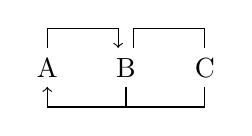
\begin{tikzpicture}
        \node (A) at (0,0) {A};
        \node (B) at (1,0) {B};
        \node (C) at (2,0) {C};

        % A -> B
        \draw[-] (A) -- (0,0.5);
        \draw[-] (0,0.5) -- (0.9, 0.5);
        \draw[->] (0.9, 0.5) -- (0.9, 0.25);

        % B -> C
        \draw[-] (1.1, 0.25) -- (1.1, 0.5);
        \draw[-] (1.1, 0.5) -- (2, 0.5);
        \draw[-] (2, 0.5) -- (C);

        % BC -> A
        \draw[-] (B) -- (1, -0.5);
        \draw[-] (C) -- (2, -0.5);
        \draw[-] (2, -0.5) -- (0, -0.5);
        \draw[->] (0, -0.5) -- (A);
    \end{tikzpicture}
\end{figure}
\FloatBarrier
\ppart{1}
Which of the following dependencies can you infer does \textit{not} hold over
scheme $S$?

(a) $A \rightarrow B$, (b) $BC \rightarrow A$, (c) $B \rightarrow C$

We'll look at the following three pictures
\begin{figure}[ht!]
    \center
    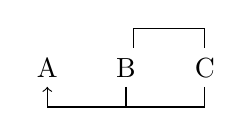
\begin{tikzpicture}
        \node (A) at (0,0) {A};
        \node (B) at (1,0) {B};
        \node (C) at (2,0) {C};

        %% A -> B
        %\draw[-] (A) -- (0,0.5);
        %\draw[-] (0,0.5) -- (0.9, 0.5);
        %\draw[->] (0.9, 0.5) -- (0.9, 0.25);

        % B -> C
        \draw[-] (1.1, 0.25) -- (1.1, 0.5);
        \draw[-] (1.1, 0.5) -- (2, 0.5);
        \draw[-] (2, 0.5) -- (C);

        % BC -> A
        \draw[-] (B) -- (1, -0.5);
        \draw[-] (C) -- (2, -0.5);
        \draw[-] (2, -0.5) -- (0, -0.5);
        \draw[->] (0, -0.5) -- (A);
    \end{tikzpicture}
\end{figure}

\begin{figure}[ht!]
    \center
    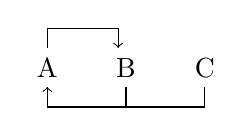
\begin{tikzpicture}
        \node (A) at (0,0) {A};
        \node (B) at (1,0) {B};
        \node (C) at (2,0) {C};

        % A -> B
        \draw[-] (A) -- (0,0.5);
        \draw[-] (0,0.5) -- (0.9, 0.5);
        \draw[->] (0.9, 0.5) -- (0.9, 0.25);

        %% B -> C
        %\draw[-] (1.1, 0.25) -- (1.1, 0.5);
        %\draw[-] (1.1, 0.5) -- (2, 0.5);
        %\draw[-] (2, 0.5) -- (C);

        % BC -> A
        \draw[-] (B) -- (1, -0.5);
        \draw[-] (C) -- (2, -0.5);
        \draw[-] (2, -0.5) -- (0, -0.5);
        \draw[->] (0, -0.5) -- (A);
    \end{tikzpicture}
\end{figure}
\begin{figure}[ht!]
    \center
    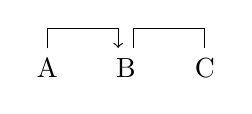
\begin{tikzpicture}
        \node (A) at (0,0) {A};
        \node (B) at (1,0) {B};
        \node (C) at (2,0) {C};

        % A -> B
        \draw[-] (A) -- (0,0.5);
        \draw[-] (0,0.5) -- (0.9, 0.5);
        \draw[->] (0.9, 0.5) -- (0.9, 0.25);

        % B -> C
        \draw[-] (1.1, 0.25) -- (1.1, 0.5);
        \draw[-] (1.1, 0.5) -- (2, 0.5);
        \draw[-] (2, 0.5) -- (C);

        %% BC -> A
        %\draw[-] (B) -- (1, -0.5);
        %\draw[-] (C) -- (2, -0.5);
        %\draw[-] (2, -0.5) -- (0, -0.5);
        %\draw[->] (0, -0.5) -- (A);
    \end{tikzpicture}
\end{figure}

We see that the third diagram is the only legal dependency, which is where the
dependency $BC \rightarrow A$ is removed. $\therefore$ (b) does \textbf{not}
hold.


\ppart{2}
Can you identify any dependencies that hold over $S$?

We are only given an instance of $S$ and can't determine what relationships hold
for \textbf{all} instances of $S$.

\problem{3}
Removed from assignment

\problem{4}
Consider relation $R = ABCDE$ with the below relationships. Convert to BCNF.

\begin{figure}[ht!]
    \center
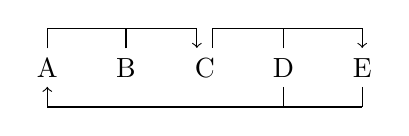
\begin{tikzpicture}
    \node (A) at (0,0) {A};
    \node (B) at (1,0) {B};
    \node (C) at (2,0) {C};
    \node (D) at (3,0) {D};
    \node (E) at (4,0) {E};

    \draw[-] (A) -- (0,0.5);
    \draw[-] (B) -- (1,0.5);
    \draw[-] (0,0.5) -- (1.9, 0.5);
    \draw[->] (1.9,0.5) -- (1.9, 0.25);

    \draw[-] (2.1, 0.25) -- (2.1, 0.5);
    \draw[-] (D) -- (3, 0.5);
    \draw[-] (2.1, 0.5) -- (4, 0.5);
    \draw[->] (4,0.5) -- (4, 0.25);

    \draw[-] (D) -- (3, -0.5);
    \draw[-] (E) -- (4, -0.5);
    \draw[-] (4,-0.5) -- (0, -0.5);
    \draw[->] (0, -0.5) -- (A);
\end{tikzpicture}
\end{figure}

\begin{figure}[ht!]
    \center
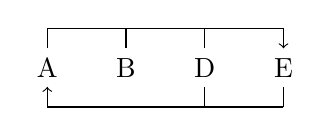
\begin{tikzpicture}
    \node (A) at (0,0) {A};
    \node (B) at (1,0) {B};
    \node (D) at (2,0) {D};
    \node (E) at (3,0) {E};

    \draw[-] (A) -- (0,0.5);
    \draw[-] (B) -- (1,0.5);
    \draw[-] (D) -- (2,0.5);
    \draw[-] (0,0.5) -- (3, 0.5);
    \draw[->] (3,0.5) -- (E);

    \draw[-] (E) -- (3, -0.5);
    \draw[-] (D) -- (2, -0.5);
    \draw[-] (3, -0.5) -- (0, -0.5);
    \draw[->] (0, -0.5) -- (A);

\end{tikzpicture}
\end{figure}

\begin{figure}[ht!]
    \center

\begin{tikzpicture}
    \node (A) at (0,0) {A};
    \node (B) at (1,0) {B};
    \node (D) at (2,0) {D};

\end{tikzpicture}
\end{figure}
\FloatBarrier

\problem{5: 19.13}
Consider a relation $R$ with five attributes $ABCDE$

\ppart{1}
For each of the following instances of R, state whether it violates (a) the FD
$BC\rightarrow D$ and (b) the MVD $BC\rightarrow\rightarrow D$
\begin{enumerate}[label=(\alph*)]
    \item \{\}  
        No. 
    \item \{($a,2,3,4,5),(2,a,3,5,5)$\} 
        $BC\rightarrow D$ is violated if $a=2$
    \item \{$(a,2,3,4,5),(2,a,3,5,5),(a,2,3,4,6)$\} $BC\rightarrow D$ and
        $BC\rightarrow\rightarrow D$ are both violated if $a=2$. We need another
        tuple that ends in $5,6$.
    \item \{$(a,2,3,4,5),(2,a,3,4,5),(a,2,3,6,5)$\}
        $BC\rightarrow D$ is violated because if $a=2$ then there is a duplicate
        row.
    \item \{$(a,2,3,4,5), (2,a,3,7,5), (a,2,3,4,6)$\}
        Both $BC\rightarrow D$ and $BC\rightarrow\rightarrow D$ are violated.
        $BC\rightarrow D$ is violated because of the second tuple.
        $BC\rightarrow\rightarrow D$ is violated because we must have another
        tuple that pairs with the second tuple.
    \item \{$(a,2,3,4,5),(2,a,3,4,5), (a,2,3,6,5), (a,2,3,6,6)$\}
        $BC\rightarrow D$ is violated because there is not a unique value
        defined by $BC$. $BC\rightarrow\rightarrow D$ is violated because the
        entry for the $D$th column in the $4^{th}$ tuple isn't the same as in
        the $1^{st}$ tuple.
    \item \{$(a,2,3,4,5),(a,2,3,6,5),(a,2,3,6,6),(a,2,3,4,6)$\}
        Just $BC\rightarrow D$ is violated because the third tuple's last entry
        isn't also a 5.
\end{enumerate}

\ppart{2}
If each instance for $R$ listed above is legal, what can you say about the DF $A
\rightarrow B$?

We cannot say anything, because there are not unique relationships.

\problem{6}
Let $R$ be a relation, $X$ a set of attributes of $R$, and $A$ an attribute of
$R$. (Also denote that $XA$ the result of adding $A$ to $X$) Define the support
of $X$, written as $\#X$, as the number of distinct tuples in $R|X$ ($R$
restricted to, or projected onto, the attributes of $X$). Prove that if $X
\rightarrow A$, then $\#X = \#XA$.

Proof by contradiction:

Let $X = BC$ such that $BC\rightarrow A$.

\FloatBarrier
\begin{figure}[ht]
    \center
\begin{tabular}{|c|c|c|}
    \hline
    A & B & C \\
    \hline
    1 & 2 & 3 \\
    \hline
    4 & 5 & 6 \\
    \hline
    7 & 2 & 3 \\
    \hline
\end{tabular}
\end{figure}
\FloatBarrier

We see here that there is a violation in the third row because $\#X = 2$ and
$\#XA = 3$. This is not a legal relationship.  We note that we only have legal
schemas if there is an injective relationship. If we have an injective
relationship (onto) then we would have the relationship $\#X \leq \#XA$ (allows
for surjection). For strict equality to hold, there needs to be a bijective
relationship.


\problem{7}
Prove that if $R$ is in 3NF and has only one candidate key, then $R$ is in BCNF.

\problem{8}
Insert the following values into an initially empty B+ tree with parameter $d=2$
and values $17, 11, 50, 22, 5, 35, 42, 60, 15, 30, 25, 27, 37, 40, 20$.

\problem{9}
Repeat the previous problem with $d=3$

\problem{10: 10.8 part 1}
Assume that you have just built a dense $B+$ tree index using Alternative (2) on
a heap file containing 20,000 records. The key field for this $B+$ tree index is
a 40-byte string, and it is a candidate key. Pointers (le., record ids and page
ids) and (at most) 10-byte values. The size of one disk page is 1000 bytes. The
index was built in a bottom-up fashion using the bulk loading algorithm, and the
nodes at each level were filled up as much as possible.

\ppart{1}
How many levels does the resulting tree have?


\end{document}
